\section{Aufbau und Durchführung}
\subsection{Aufbau}
\label{sec:Aufbau}
\subsubsection{Erzeugung der Isotope}
Dazu befinden sich die Proben in einem Behälter wie er in Abbildung \ref{abb:1} gezeigt wird.
\begin{figure}[H]
  \centering
  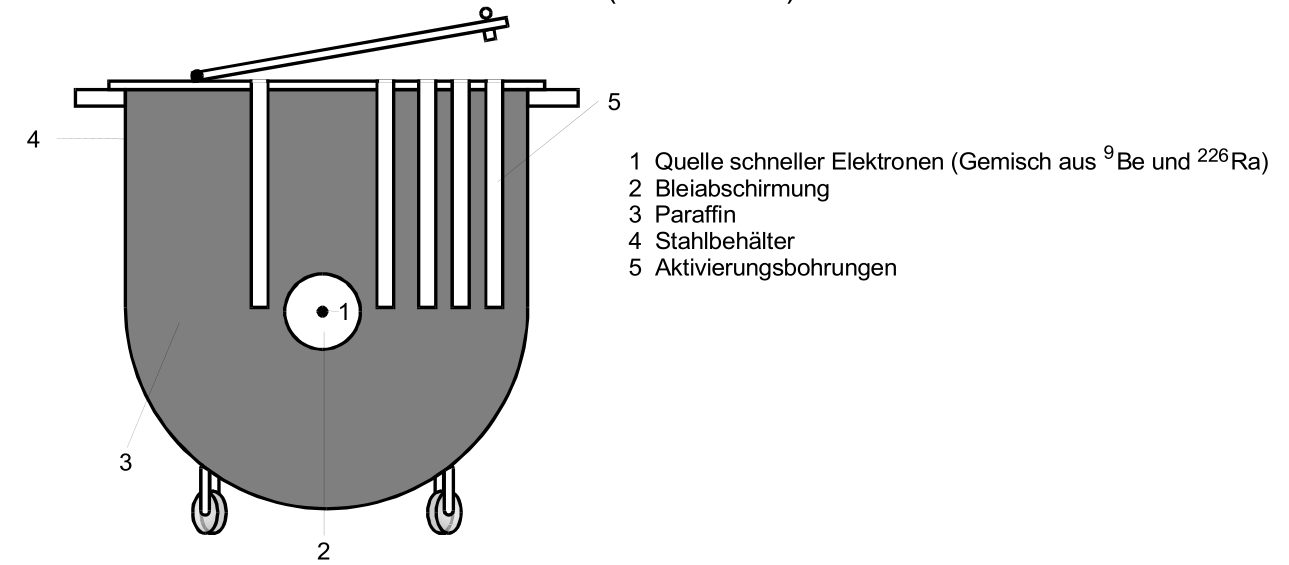
\includegraphics[height=6cm]{ressources/erzeugung.png}
  \caption{Erzeugung der Isotope. \cite{skript}}
  \label{abb:1}
\end{figure}
In dessen Zentrum befindet sich Radium und Berylium.
Die Alpha-Strahlen des Radiums sorgen dafür, dass das Berylium Neutronen emittiert, welche dann durch eine Parafinwand diffundieren und dadurch schließlich niederenergetisch auf die Proben stoßen.
Diese werden in diesem Prozess zu Isotopen, welche für den Versuch verwendet werden können.


\subsubsection{Untersuchung der Isotope}
Zur Untersuchung der Halbwertszeiten der Isotope wird ein einfacher Aufbau, dargestellt in Abbildung \ref{abb:2}, verwendet.
\begin{figure}[H]
  \centering
  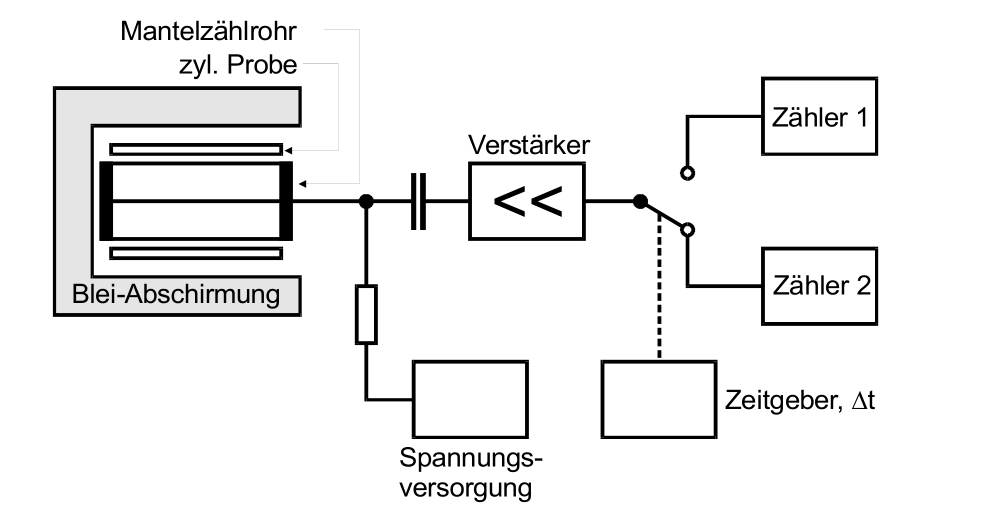
\includegraphics[height=6cm]{ressources/aufbau.png}
  \caption{Versuchsaufbau zur Untersuchung der Zerfallsprozesse. \cite{skript}}
  \label{abb:2}
\end{figure}
Der Aufbau spiegelt prinzipiell ein Geigermüllerzählrohr wieder.
Die Probe hüllt hierbei ein Mantelzählrohr ein.
Es handelt sich um einen mit Argon befüllten zylindrischen Behälter, welcher von einer positiv geladenen Anode durchlaufen wird.
Der Mantel ist negativ geladen, wodurch, wenn ein Strahlungsquant ein Argonatom ionisiert, eine Kettenreaktion von Ionisationsprozessen gestartet wird, die in einem Stromimpuls resultiert.
Diese werden von zwei Zählern abwechselnd in einem Zeitintervall, welches durch einen Zeitgeber eingestellt werden kann, gezählt.
Zur Abschirmung der Strahlung sind Probe und Mantelzählrohr von Bleiwänden umgeben.
